
%%==========================================================
\chapter{Límites y Continuidad}
%%==========================================================

El concepto de límite marca la transición del álgebra clásica al análisis
matemático. Inicialmente, Newton y Leibniz basaron el cálculo en intuiciones
sobre cantidades infinitamente pequeñas, lo que provocó críticas por falta
de rigor, como las de Berkeley en \emph{The Analyst} (1734), quien calificó
los infinitésimos de \emph{fantasmas de cantidades que desaparecen}. La
formalización llegó con Cauchy (1821), quien definió el límite como un proceso
de aproximación, y se consolidó con Weierstrass mediante la rigurosa definición
$\varepsilon$-$\delta$. Esta precisión permitió distinguir claramente entre
\emph{acercarse} a un valor y el valor mismo, sentando las bases del análisis
moderno.

\begin{rem}
La historia del análisis muestra cómo la intuición práctica suele preceder
al rigor formal. Se recomienda complementar este capítulo con los enfoques
de Purcell, Spivak y Larson, citados en la bibliografía.
\end{rem}

Informalmente, $\lim_{x\to a}f(x)=L$ significa que $f(x)$ se aproxima a $L$
tanto como se desee cuando $x$ se acerca a $a$, \emph{sin necesidad de que
$x=a$}. Esta condición es crucial: el límite describe el comportamiento
\emph{alrededor} de $a$, no en $a$. Así, una función puede tener límite en
puntos donde no está definida o donde su valor es distinto.

\begin{example}[Discontinuidad evitable en $f(x)=(x^2-1)/(x-1)$]
Calcule $\displaystyle\lim_{x\to 1}\frac{x^2-1}{x-1}$.

\begin{myproof}
\textbf{Paso 1: Simplificar para $x\neq 1$.} La función no está definida en $x=1$, pero para $x\neq 1$:
\[
  \frac{x^2-1}{x-1} = \frac{(x-1)(x+1)}{x-1} = x+1.
\]

\textbf{Paso 2: Calcular el límite.} Al acercarse a $1$, $f(x)=x+1\to 2$:
\[
  \boxed{\lim_{x\to 1}\frac{x^2-1}{x-1} = 2,}
\]
aunque $f(1)$ no exista. La figura~\ref{fig:limite_ejemplo} ilustra este comportamiento:

\begin{figure}[H]
  \centering
  \begin{tikzpicture}
    \begin{axis}[scale=0.7,
      axis lines   = middle,
      xlabel       = {$x$},
      ylabel       = {$f(x)$},
      domain       = -2:3,
      samples      = 100,
      ymin = -1, ymax = 4,
      xmin = -2, xmax = 3,
      grid         = major,
      width        = 0.7\textwidth,
      title        = {$f(x)=\dfrac{x^2-1}{x-1}=x+1$ para $x\neq 1$}
    ]
      \addplot[blue, thick] {x + 1};
      \addplot[only marks, mark=*,
               mark options={fill=white, draw=blue, line width=1.5pt},
               mark size=4pt]
        coordinates {(1,2)};
      \node[pin=above right:{Límite $= 2$}] at (axis cs:1,2) {};
    \end{axis}
  \end{tikzpicture}
  \caption{Representación gráfica de la discontinuidad evitable en $x=1$.}
  \label{fig:limite_ejemplo}
\end{figure}
\end{myproof}
\end{example}

%%==========================================================
\section{Definición Formal: Épsilon-Delta}
%%==========================================================

El trabajo de Weierstrass permite definir este concepto de manera formal:

\begin{definition}
Sea $f$ definida en un intervalo abierto que contiene a $c$, excepto quizás
en $c$ mismo. Se dice que
\(
  \lim_{x \to c} f(x) = L
\)
si para todo $\epsilon > 0$ existe $\delta > 0$ tal que
\[
  0 < |x - c| < \delta \implies |f(x) - L| < \epsilon.
\]
\end{definition}

Esta definición traduce la noción intuitiva de ``acercarse'' a una condición
cuantitativa. El valor $\epsilon$ fija una tolerancia vertical en la imagen,
mientras que $\delta$ determina la proximidad horizontal requerida en el dominio
para cumplirla. La condición $0<|x-c|$ recalca que el comportamiento de $f$
\emph{exactamente} en $c$ es irrelevante; solo importa su entorno perforado.
La figura~\ref{fig:limite_epsilon_delta} representa la condición en general.

\begin{figure}[H]
\centering
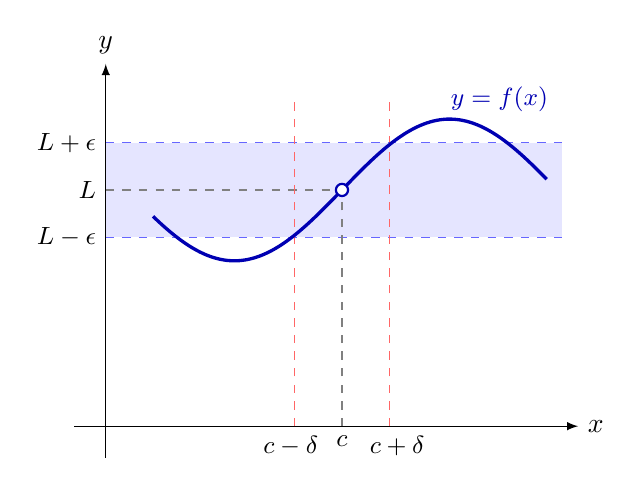
\begin{tikzpicture}[>=latex, scale=1.0]
  % Ejes
  \draw[->] (-0.4,0) -- (6,0) node[right] {$x$};
  \draw[->] (0,-0.4) -- (0,4.6) node[above] {$y$};
  % Banda epsilon (horizontal)
  \fill[blue!10] (0,2.4) rectangle (5.8,3.6);
  \draw[blue!60, dashed] (0,2.4) -- (5.8,2.4);
  \draw[blue!60, dashed] (0,3.6) -- (5.8,3.6);
  \node[left, font=\small] at (0,3.6) {$L+\epsilon$};
  \node[left, font=\small] at (0,3.0) {$L$};
  \node[left, font=\small] at (0,2.4) {$L-\epsilon$};
  \draw[gray, dashed] (0,3.0) -- (3,3.0);
  % Entorno delta (vertical)
  \draw[red!60, dashed] (2.4,0) -- (2.4,4.2);
  \draw[red!60, dashed] (3.6,0) -- (3.6,4.2);
  \node[below, font=\small] at (2.35,0) {$c-\delta$};
  \node[below, font=\small] at (3,0) {$c$};
  \node[below, font=\small] at (3.7,0) {$c+\delta$};
  \draw[gray, dashed] (3,0) -- (3,3.0);
  % Curva
  \draw[blue!70!black, very thick, domain=0.6:5.6, smooth, samples=60]
      plot (\x, {3 + 0.9*sin(deg(1.15*(\x-3)))});
  \node[blue!70!black, font=\small] at (5.0,4.15) {$y=f(x)$};
  % Punto excluido en (c, L)
  \fill[white] (3,3) circle (2.2pt);
  \draw[blue!70!black, thick] (3,3) circle (2.2pt);
\end{tikzpicture}
\caption{Definición $\epsilon$-$\delta$: fijada la tolerancia $\epsilon$
alrededor de $L$ (banda horizontal), existe $\delta$ tal que todo $x$ del
entorno perforado $(c-\delta,\,c+\delta)$ tiene imagen dentro de la banda.
El valor $f(c)$, si existe, es irrelevante (punto excluido).}
\label{fig:limite_epsilon_delta}
\end{figure}

\begin{rem}
Puede interpretarse como un \textbf{juego adversarial}: un ``retador'' elige
un $\epsilon>0$ arbitrario y el ``defensor'' debe hallar un $\delta>0$ que
satisfaga la implicación. Si el defensor siempre puede responder, sin importar
cuán pequeño sea $\epsilon$, el límite es $L$. Esta analogía, destacada por
Spivak~\cite{spivak2012calculus}, es una herramienta pedagógica poderosa para
asimilar el concepto.
\end{rem}

\begin{example}[Demostración $\epsilon$-$\delta$: $\protect\lim_{x\to 3}(2x-1)=5$]
Demostrar que $\lim_{x \to 3}(2x-1) = 5$ mediante la definición
$\epsilon$-$\delta$.

\begin{myproof}
\textbf{Paso 1: Análisis preliminar.} Se busca $\delta>0$ tal que
\[
  0 < |x-3| < \delta \implies |(2x-1)-5| < \epsilon.
\]
Observamos que $|(2x-1)-5| = |2x-6| = 2|x-3|$. Para garantizar
$2|x-3| < \epsilon$, basta exigir $|x-3| < \epsilon/2$.

\textbf{Paso 2: Demostración formal.} Elegimos $\delta = \epsilon/2$
(figura~\ref{fig:epsilon_delta_demo}). Entonces, si $0 < |x-3| < \delta$:
\[
  |(2x-1)-5| = 2|x-3| < 2\cdot\frac{\epsilon}{2} = \epsilon.
\]
\[
  \boxed{\lim_{x\to 3}(2x-1) = 5.}
\]

\begin{figure}[H]
\centering
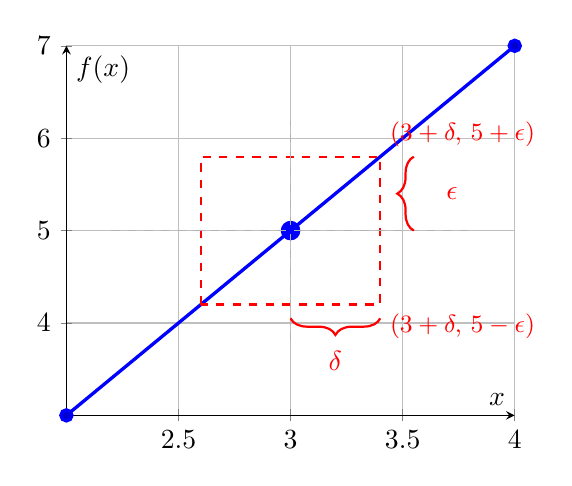
\begin{tikzpicture}
  \begin{axis}[
    axis lines  = middle,
    xlabel      = {$x$},
    ylabel      = {$f(x)$},
    xmin = 2, xmax = 4,
    ymin = 3,   ymax = 7,
    grid        = major,
    width       = 0.6\textwidth,
    samples     = 2,
    domain      = 2:4,
    clip        = false,
    every axis plot/.append style={blue, very thick}
  ]
    \addplot {2*x - 1};
    \node[fill=blue, circle, inner sep=2.5pt] at (axis cs:3,5) {};

    \def\ep{0.8}
    \def\del{0.4}
    \def\cx{3}
    \def\cy{5}

    \draw[red, dashed, thick]
      (\cx-\del, \cy-\ep) rectangle (\cx+\del, \cy+\ep);

    \draw[gray!60, dashed]
      (\cx, \cy-\ep-0.4) -- (\cx, \cy+\ep+0.4);
    \draw[gray!60, dashed]
      (\cx-\del-0.4, \cy) -- (\cx+\del+0.4, \cy);

    \draw[decorate,
          decoration={brace, amplitude=6pt},
          thick, red]
      (\cx+\del+0.15, \cy) -- (\cx+\del+0.15, \cy+\ep)
      node[midway, right, xshift=8pt] {$\epsilon$};

    \draw[decorate,
          decoration={brace, amplitude=6pt, mirror},
          thick, red]
      (\cx, \cy-\ep-0.15) -- (\cx+\del, \cy-\ep-0.15)
      node[midway, below, yshift=-8pt] {$\delta$};

    \node[red, font=\small] at (\cx+\del, \cy+\ep)
      [above right] {$(3+\delta,\, 5+\epsilon)$};
    \node[red, font=\small] at (\cx+\del, \cy-\ep)
      [below right] {$(3+\delta,\, 5-\epsilon)$};
  \end{axis}
\end{tikzpicture}
\caption{Interpretación geométrica de la demostración: la banda
$5\pm\epsilon$ y el entorno $3\pm\delta$ con $\delta=\epsilon/2$.}
\label{fig:epsilon_delta_demo}
\end{figure}
\end{myproof}
\end{example}

\begin{theorem}[Unicidad del límite]
Si $\lim_{x\to c}f(x)$ existe, entonces es único.
\end{theorem}

\begin{proof}
Supongamos, por contradicción, que existen dos límites distintos $L_1 \neq L_2$.
Sea $\epsilon = \dfrac{|L_1-L_2|}{2} > 0$. Por la definición, existen
$\delta_1, \delta_2 > 0$ tales que:
\[
  0<|x-c|<\delta_1 \implies |f(x)-L_1|<\epsilon, \qquad
  0<|x-c|<\delta_2 \implies |f(x)-L_2|<\epsilon.
\]
Tomando $\delta = \min\{\delta_1, \delta_2\}$, para cualquier $x$ con
$0<|x-c|<\delta$ se cumplen ambas desigualdades. Aplicando la desigualdad
triangular:
\[
  |L_1-L_2| \leq |L_1-f(x)| + |f(x)-L_2| < \epsilon + \epsilon
             = 2\epsilon = |L_1-L_2|,
\]
lo cual es absurdo. Por tanto, $L_1 = L_2$.
\end{proof}

%%==========================================================
\section{Propiedades Algebraicas de los Límites}
%%==========================================================

Los límites satisfacen las siguientes propiedades algebraicas:

\begin{theorem}[Leyes de los límites]
Sean $\lim_{x\to c}f(x) = L$ y $\lim_{x\to c}g(x) = K$, con $k\in\R$:
\begin{enumerate}
  \item $\displaystyle\lim_{x\to c} k = k$.
  \item $\displaystyle\lim_{x\to c}\bigl[f(x)\pm g(x)\bigr] = L \pm K$.
  \item $\displaystyle\lim_{x\to c}\bigl[k\cdot f(x)\bigr] = kL$.
  \item $\displaystyle\lim_{x\to c}\bigl[f(x)\cdot g(x)\bigr] = LK$.
  \item $\displaystyle\lim_{x\to c}\frac{f(x)}{g(x)} = \frac{L}{K}$,\quad
        siempre que $K\neq 0$.
  \item $\displaystyle\lim_{x\to c}\bigl[f(x)\bigr]^n = L^n$,\quad
        $n\in\N$.
  \item $\displaystyle\lim_{x\to c}\sqrt[n]{f(x)} = \sqrt[n]{L}$,\quad
        con $L>0$ si $n$ es par.
\end{enumerate}
\end{theorem}

\begin{rem}
Gracias a estas propiedades, el límite de cualquier función polinómica
\[
  p(x) = a_n x^n + \cdots + a_0
\]
en un punto $c$ se reduce simplemente a evaluar $p(c)$. Esto justifica el
procedimiento de \textbf{sustitución directa} que se utiliza en la gran
mayoría de los cálculos elementales.
\end{rem}

En muchas funciones de interés práctico como la función valor absoluto,
la función piso o las funciones definidas por casos el comportamiento
difiere según si $x$ se acerca por valores menores o mayores que $c$.

\begin{definition}[Límites laterales]
$L$ es el \textbf{límite por la derecha} de $f$ en $c$,
$\lim_{x\to c^+}f(x)=L$, si para todo $\epsilon>0$ existe $\delta>0$ tal
que $0<x-c<\delta$ implica $|f(x)-L|<\epsilon$. Análogamente,
$\lim_{x\to c^-}f(x)=L$ si $0<c-x<\delta$ implica $|f(x)-L|<\epsilon$.
\end{definition}

\begin{theorem}[Condición de existencia del límite bilateral]
$\lim_{x\to c}f(x) = L$ si y solo si
$\lim_{x\to c^-}f(x) = L$ \;y\; $\lim_{x\to c^+}f(x) = L$.
\end{theorem}

\begin{example}[Límite lateral de $|x|/x$ en $x=0$]
Calcular $\displaystyle\lim_{x\to 0}\frac{|x|}{x}$.

\begin{myproof}
\textbf{Paso 1: Límite por la derecha.} Para $x>0$, $|x|=x$, luego
\[
  \lim_{x\to 0^+}\frac{|x|}{x} = \lim_{x\to 0^+}\frac{x}{x} = 1.
\]

\textbf{Paso 2: Límite por la izquierda.} Para $x<0$, $|x|=-x$, luego
\[
  \lim_{x\to 0^-}\frac{|x|}{x} = \lim_{x\to 0^-}\frac{-x}{x} = -1.
\]

\textbf{Paso 3: Conclusión.} Como los límites laterales difieren:
\[
  \boxed{\lim_{x\to 0}\frac{|x|}{x} \;\text{no existe.}}
\]
\end{myproof}
\end{example}

\begin{example}[Límite de función definida por partes en $x=2$]
Sea
\[
  f(x) =
  \begin{cases}
    x^2+1 & \text{si } x < 2,\\
    3x-1  & \text{si } x \geq 2.
  \end{cases}
\]
Determinar si $\lim_{x\to 2}f(x)$ existe.

\begin{myproof}
\textbf{Paso 1: Límite por la izquierda.}
\[
  \lim_{x\to 2^-}f(x) = \lim_{x\to 2^-}(x^2+1) = 4+1 = 5.
\]

\textbf{Paso 2: Límite por la derecha.}
\[
  \lim_{x\to 2^+}f(x) = \lim_{x\to 2^+}(3x-1) = 6-1 = 5.
\]

\textbf{Paso 3: Conclusión.} Como ambos límites laterales coinciden:
\[
  \boxed{\lim_{x\to 2}f(x) = 5.}
\]
\end{myproof}
\end{example}

\begin{example}[Límite por racionalización]
Calcular $\displaystyle\lim_{x\to 1}\frac{\sqrt{x}-1}{x-1}$.

\begin{myproof}
\textbf{Paso 1: Reconocer la indeterminación.} Numerador y denominador se
anulan en $x=1$: es una forma $0/0$ con radical, que se trata multiplicando
por el conjugado del numerador.

\textbf{Paso 2: Racionalizar.} Para $x\neq 1$:
\[
  \frac{\sqrt{x}-1}{x-1}
  = \frac{(\sqrt{x}-1)(\sqrt{x}+1)}{(x-1)(\sqrt{x}+1)}
  = \frac{x-1}{(x-1)(\sqrt{x}+1)}
  = \frac{1}{\sqrt{x}+1}.
\]

\textbf{Paso 3: Evaluar.} La última expresión es continua en $x=1$:
\[
  \boxed{\lim_{x\to 1}\frac{\sqrt{x}-1}{x-1}
  = \frac{1}{\sqrt{1}+1} = \frac{1}{2}.}
\]
\end{myproof}
\end{example}

%%==========================================================
\section{El Teorema del Encaje}
%%==========================================================

Este teorema permite calcular varios límites y es la base de múltiples
demostraciones.

\begin{theorem}[Del encaje o del sándwich]
Si $h(x)\leq f(x)\leq g(x)$ en algún intervalo abierto que contiene a
$c$ (salvo posiblemente en $c$), y
\(
  \lim_{x\to c}h(x) = \lim_{x\to c}g(x) = L,
\)
entonces $\lim_{x\to c}f(x)=L$.
\end{theorem}

La idea geométrica es transparente: si $f$ queda permanentemente comprimida
entre $h$ y $g$ que convergen al mismo valor, $f$ tampoco tiene escapatoria.
Su aplicación más célebre es el límite trigonométrico fundamental.

\begin{theorem} Demuestre que \(
  \lim_{x \to 0} \frac{\sen x}{x} = 1.
\)
\end{theorem}

\begin{proof}
Sea $0<x<\dfrac{\pi}{2}$. Considérese el círculo unitario centrado en el
origen y los puntos $O=(0,0)$, $A=(1,0)$, $B=(\cos x,\sen x)$ sobre dicho
círculo, y $T=(1,\tan x)$ sobre la recta $x=1$ (véase la
figura~\ref{fig:encaje_areas}).

\begin{figure}[H]
\centering
\begin{tikzpicture}[scale=3.5, >=stealth, line cap=round, line join=round]
  \pgfmathsetmacro{\ang}{38}
  \pgfmathsetmacro{\cosA}{cos(\ang)}
  \pgfmathsetmacro{\sinA}{sin(\ang)}
  \pgfmathsetmacro{\tanA}{tan(\ang)}

  % Rellenos (de atrás hacia adelante)
  \fill[orange!14]  (0,0) -- (1,0) -- (1,\tanA) -- cycle;
  \fill[teal!22]    (0,0) -- (1,0)
        arc[start angle=0, end angle=\ang, radius=1] -- cycle;
  \fill[blue!20]    (0,0) -- (1,0) -- (\cosA,\sinA) -- cycle;

  % Círculo unitario (guía tenue)
  \draw[gray!35, very thin] (0,0) circle[radius=1];

  % Arco AB sobre el círculo
  \draw[teal!65!black, thick]
        (1,0) arc[start angle=0, end angle=\ang, radius=1];

  % Lados de los triángulos
  \draw[thick] (0,0)       -- (1,0);
  \draw[thick] (0,0)       -- (\cosA,\sinA);
  \draw[thick] (0,0)       -- (1,\tanA);
  \draw[thick] (1,0)       -- (1,\tanA);

  % Segmento auxiliar (perpendicular desde B al eje x)
  \draw[dashed, gray!70] (\cosA,0) -- (\cosA,\sinA);

  % Marca de ángulo recto en A
  \draw[thin] (1,0.038) -- (0.962,0.038) -- (0.962,0);

  % Arco del ángulo x
  \draw[->] (0.21,0) arc[start angle=0, end angle=\ang, radius=0.21];
  \node[font=\small] at ({0.30*cos(\ang/2)},{0.30*sin(\ang/2)}) {$x$};

  % Ejes
  \draw[->] (-0.12,0) -- (1.28,0);
  \draw[->] (0,-0.10) -- (0,\tanA+0.16);

  % Puntos notables
  \fill (0,0)         circle[radius=0.65pt];
  \fill (1,0)         circle[radius=0.65pt];
  \fill (\cosA,\sinA) circle[radius=0.65pt];
  \fill (1,\tanA)     circle[radius=0.65pt];

  % Etiquetas de puntos
  \node[below left,  font=\small] at (0,0)          {$O$};
  \node[below,       font=\small] at (1,-0.025)      {$A$};
  \node[above left,  font=\small] at (\cosA,\sinA)   {$B$};
  \node[right,       font=\small] at (1,\tanA)       {$T$};

  % Etiquetas de segmentos
  \node[below, font=\scriptsize, gray!80!black]
        at (\cosA/2,-0.055) {$\cos x$};
  \node[right, font=\scriptsize, gray!80!black]
        at (\cosA+0.02,\sinA/2) {$\sen x$};
  \node[right, font=\scriptsize, gray!80!black]
        at (1.03,\tanA/2) {$\tan x$};

  % Etiquetas de áreas
  \node[font=\scriptsize, blue!70!black]
        at ({(1+\cosA)/3+0.04},{\sinA/4})
        {$\tfrac{1}{2}\sen x$};
  \node[font=\scriptsize, teal!70!black]
        at ({0.55*cos(\ang/2+5)},{0.55*sin(\ang/2+5)})
        {$\tfrac{x}{2}$};
  \node[font=\scriptsize, orange!75!black]
        at (0.82,\tanA*0.82)
        {$\tfrac{1}{2}\tan x$};
\end{tikzpicture}
\caption{Comparación de áreas: triángulo inscrito $\subset$ sector $\subset$
triángulo circunscrito.}
\label{fig:encaje_areas}
\end{figure}

\noindent Comparando las tres áreas coloreadas se obtiene la cadena
\[
  \underbrace{\tfrac{1}{2}\sen x}_{\triangle\,OAB}
  \;\leq\;
  \underbrace{\tfrac{x}{2}}_{\text{sector}}
  \;\leq\;
  \underbrace{\tfrac{1}{2}\tan x}_{\triangle\,OAT}.
\]
Dividiendo por $\dfrac{1}{2}\sen x > 0$ y usando que
$\tan x = \sen x/\cos x$:
\[
  1 \;\leq\; \frac{x}{\sen x} \;\leq\; \frac{1}{\cos x}.
\]
Tomando recíprocos (lo que invierte las desigualdades):
\[
  \cos x \;\leq\; \frac{\sen x}{x} \;\leq\; 1.
\]
Como $\displaystyle\lim_{x\to 0^+}\cos x = 1$, el Teorema del Encaje da
\[
  \lim_{x\to 0^+}\frac{\sen x}{x}=1.
\]
La función $f(x)=\dfrac{\sen x}{x}$ es par (pues $\sen(-x)=-\sen x$), de
modo que $f(-x)=f(x)$ y, en consecuencia,
\[
  \lim_{x\to 0^-}\frac{\sen x}{x}
  = \lim_{x\to 0^+}\frac{\sen(-x)}{-x}
  = \lim_{x\to 0^+}\frac{\sen x}{x} = 1.
\]
Al coincidir ambos límites laterales se concluye
\(
  \lim_{x \to 0} \frac{\sen x}{x} = 1.
\)
\end{proof}

\begin{rem}
Como corolario inmediato, usando la identidad $1-\cos x = 2\sen^2\!\frac{x}{2}$,
se puede demostrar que $\lim_{x\to 0}\dfrac{1-\cos x}{x} = 0$. Estos dos
límites son la base sobre la que se construyen las fórmulas de derivación de
$\sen x$ y $\cos x$.
\end{rem}

%%==========================================================
\section{Límites Infinitos y en el Infinito}
%%==========================================================

\begin{definition}
Se dice que $\lim_{x\to c}f(x) = +\infty$ si para todo $M>0$ existe
$\delta>0$ tal que $0<|x-c|<\delta$ implica $f(x)>M$. Geométricamente,
la recta $x=c$ es una \textbf{asíntota vertical} de la gráfica de $f$.

Se dice que $\lim_{x\to\infty}f(x) = L$ si para todo $\epsilon>0$ existe
$N>0$ tal que $x>N$ implica $|f(x)-L|<\epsilon$. En este caso, la recta
$y=L$ es una \textbf{asíntota horizontal}.
\end{definition}

\begin{rem}
El comportamiento de funciones racionales proporciona los ejemplos más
instructivos. En $f(x)=\dfrac{1}{x-2}$, los valores crecen sin cota cuando
$x\to 2$, generando una asíntota vertical en $x=2$. En cambio,
$\lim_{x\to\infty}\dfrac{1}{x-2}=0$ da la asíntota horizontal $y=0$
(figura~\ref{fig:asintotas}).

Para funciones racionales $\dfrac{P(x)}{Q(x)}$, el comportamiento en el
infinito está completamente determinado por la relación entre los grados de
$P$ y $Q$:
\begin{itemize}
  \item Si $\deg P < \deg Q$: asíntota horizontal $y=0$.
  \item Si $\deg P = \deg Q$: asíntota horizontal $y=\dfrac{a_n}{b_n}$
        (cociente de coeficientes líderes).
  \item Si $\deg P > \deg Q$: no hay asíntota horizontal.
\end{itemize}
\end{rem}

\begin{figure}[H]
\centering
\begin{tikzpicture}
\begin{axis}[
    axis lines=middle, xlabel={$x$}, ylabel={$y$},
    xmin=-2.5, xmax=6.5, ymin=-4, ymax=4,
    width=11cm, height=6.5cm, samples=150,
    restrict y to domain=-4:4,
]
\addplot[blue, ultra thick, domain=-2.5:1.72] {1/(x-2)};
\addplot[blue, ultra thick, domain=2.28:6.4] {1/(x-2)};
\draw[red, dashed, thick] (axis cs:2,-4) -- (axis cs:2,4);
\node[red, font=\small, anchor=west] at (axis cs:2.15,3.4) {$x=2$};
\node[gray, font=\small, anchor=south] at (axis cs:5.3,0.1) {$y=0$};
\node[blue, font=\small, anchor=west] at (axis cs:4.2,1.3)
  {$f(x)=\dfrac{1}{x-2}$};
\end{axis}
\end{tikzpicture}
\caption{$f(x)=1/(x-2)$: asíntota vertical $x=2$ (los valores crecen sin
cota al acercarse a $2$) y asíntota horizontal $y=0$ (la función se aplana
hacia el eje $x$ cuando $x\to\pm\infty$).}
\label{fig:asintotas}
\end{figure}

\begin{example}[Límite en el infinito de una función racional]
Calcular $\displaystyle\lim_{x\to\infty}\frac{5x^2}{3x^2-5}$.

\begin{myproof}
\textbf{Paso 1: Identificar la estrategia.} Numerador y denominador tienen
el mismo grado: se divide entre la potencia dominante $x^2$.

\textbf{Paso 2: Dividir entre $x^2$.}
\[
  \frac{5x^2}{3x^2-5} = \frac{5}{3-\dfrac{5}{x^2}}.
\]

\textbf{Paso 3: Evaluar.} Como $5/x^2\to 0$ cuando $x\to\infty$:
\[
  \boxed{\lim_{x\to\infty}\frac{5x^2}{3x^2-5} = \frac{5}{3},}
\]
en acuerdo con la regla de los grados (cociente de coeficientes líderes).
La recta $y=5/3$ es asíntota horizontal de la gráfica.
\end{myproof}
\end{example}

\begin{example}[Asíntotas de una función racional]
Encuentre todas las asíntotas verticales y horizontales de
$f(x)=\dfrac{x^2}{16-x^2}$, verificando el tipo de infinito en cada una.

\begin{myproof}
\textbf{Paso 1: Asíntotas verticales.} El denominador $16-x^2=(4-x)(4+x)$
se anula en $x=\pm 4$, donde el numerador vale $16\neq 0$: ambas rectas son
asíntotas verticales. Análisis de signos cerca de $x=4$: si $x\to 4^-$,
entonces $16-x^2\to 0^+$ y $f(x)\to +\infty$; si $x\to 4^+$, entonces
$16-x^2\to 0^-$ y $f(x)\to -\infty$. Como $f$ es par ($f(-x)=f(x)$), cerca
de $x=-4$ los papeles se invierten: $f(x)\to -\infty$ si $x\to -4^-$ y
$f(x)\to +\infty$ si $x\to -4^+$.

\textbf{Paso 2: Asíntota horizontal.} Dividiendo entre $x^2$:
\[
  \lim_{x\to\pm\infty}\frac{x^2}{16-x^2}
  = \lim_{x\to\pm\infty}\frac{1}{\dfrac{16}{x^2}-1} = -1.
\]

\textbf{Paso 3: Conclusión.}
\[
  \boxed{\text{AV: } x=4 \text{ y } x=-4; \qquad \text{AH: } y=-1.}
\]
\end{myproof}
\end{example}

\begin{example}[Límite de tipo $1^\infty$]
Calcular $\displaystyle\lim_{x\to 0}(1+x^2)^{\cot^2 x}$.

\begin{myproof}
\textbf{Paso 1: Reconocer la forma.} La base tiende a $1$ y el exponente a
$+\infty$: forma indeterminada $1^\infty$. Se resuelve con el límite
fundamental $e = \lim_{u\to 0}(1+u)^{1/u}$.

\textbf{Paso 2: Reescribir con la estructura de $e$.}
\[
  (1+x^2)^{\cot^2 x}
  = \Bigl[(1+x^2)^{1/x^2}\Bigr]^{x^2\cot^2 x}.
\]
La expresión entre corchetes tiende a $e$ (con $u=x^2\to 0$); resta
calcular el límite del exponente.

\textbf{Paso 3: Límite del exponente.} Usando $\dfrac{x}{\sen x}\to 1$:
\[
  x^2\cot^2 x = \left(\frac{x}{\sen x}\right)^{\!2}\cos^2 x
  \;\longrightarrow\; 1^2\cdot 1 = 1.
\]

\textbf{Paso 4: Conclusión.}
\[
  \boxed{\lim_{x\to 0}(1+x^2)^{\cot^2 x} = e^{1} = e.}
\]
\end{myproof}
\end{example}

%%==========================================================
\section{Continuidad}
%%==========================================================

\begin{definition}
$f$ es \textbf{continua en $c$} si se satisfacen simultáneamente:
\begin{enumerate}
  \item $f(c)$ está definida.
  \item $\lim_{x\to c}f(x)$ existe.
  \item $\lim_{x\to c}f(x) = f(c)$.
\end{enumerate}
Si alguna condición falla, $f$ es \textbf{discontinua} en $c$. $f$ es
continua en un intervalo cerrado $[a,b]$ si es continua en $(a,b)$, y además
$\lim_{x\to a^+}f(x)=f(a)$ y $\lim_{x\to b^-}f(x)=f(b)$.
\end{definition}

La imagen intuitiva de continuidad ``se puede trazar la gráfica sin
levantar el lápiz'' captura bien la idea pero es insuficiente como
definición matemática. Nótese que la continuidad en $[a,b]$ requiere
únicamente límites laterales en los extremos, lo cual permite que funciones
como $f(x)=\sqrt{x}$ sean continuas en $[0,+\infty)$.

\begin{definition}
Sea $f$ discontinua en $c$. Se distinguen:
\begin{itemize}
  \item \textbf{Removible:} $\lim_{x\to c}f(x)$ existe pero es distinto de
        $f(c)$, o bien $f(c)$ no está definida. Se elimina redefiniendo
        $f(c):=\lim_{x\to c}f(x)$.
  \item \textbf{De salto:} los límites laterales existen pero
        $\lim_{x\to c^-}f(x)\neq\lim_{x\to c^+}f(x)$. El \emph{salto} mide
        \[
          \left|\lim_{x\to c^+}f(x) - \lim_{x\to c^-}f(x)\right|.
        \]
  \item \textbf{Infinita:} al menos un límite lateral es $\pm\infty$;
        corresponde a una asíntota vertical.
  \item \textbf{Oscilante:} el límite no existe por oscilación sin
        convergencia, como $\sen\!\left(\dfrac{1}{x}\right)$ en $x=0$.
\end{itemize}
\end{definition}

La figura~\ref{fig:tipos_discontinuidad} esquematiza los tres tipos que
aparecen con mayor frecuencia en este curso.

\begin{figure}[H]
\centering
\begin{minipage}{0.32\textwidth}
\centering
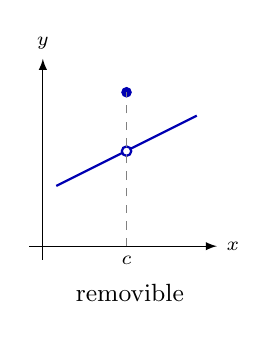
\begin{tikzpicture}[>=latex, scale=0.85]
  \draw[->] (-0.2,0) -- (2.6,0) node[right,font=\scriptsize] {$x$};
  \draw[->] (0,-0.2) -- (0,2.8) node[above,font=\scriptsize] {$y$};
  \draw[blue!70!black, thick] (0.2,0.9) -- (2.3,1.95);
  \fill[white] (1.25,1.42) circle (2pt);
  \draw[blue!70!black, thick] (1.25,1.42) circle (2pt);
  \filldraw[blue!70!black] (1.25,2.3) circle (2pt);
  \draw[dashed, gray] (1.25,0) -- (1.25,2.3);
  \node[below, font=\scriptsize] at (1.25,0) {$c$};
  \node[font=\small] at (1.3,-0.7) {removible};
\end{tikzpicture}
\end{minipage}
\hfill
\begin{minipage}{0.32\textwidth}
\centering
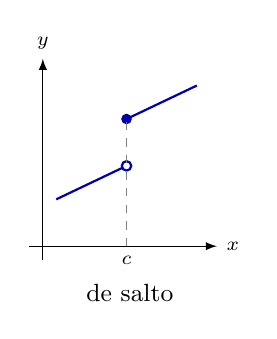
\begin{tikzpicture}[>=latex, scale=0.85]
  \draw[->] (-0.2,0) -- (2.6,0) node[right,font=\scriptsize] {$x$};
  \draw[->] (0,-0.2) -- (0,2.8) node[above,font=\scriptsize] {$y$};
  \draw[blue!70!black, thick] (0.2,0.7) -- (1.25,1.2);
  \fill[white] (1.25,1.2) circle (2pt);
  \draw[blue!70!black, thick] (1.25,1.2) circle (2pt);
  \draw[blue!70!black, thick] (1.25,1.9) -- (2.3,2.4);
  \filldraw[blue!70!black] (1.25,1.9) circle (2pt);
  \draw[dashed, gray] (1.25,0) -- (1.25,1.9);
  \node[below, font=\scriptsize] at (1.25,0) {$c$};
  \node[font=\small] at (1.3,-0.7) {de salto};
\end{tikzpicture}
\end{minipage}
\hfill
\begin{minipage}{0.32\textwidth}
\centering
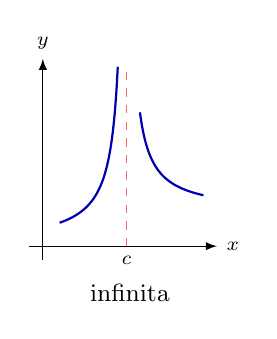
\begin{tikzpicture}[>=latex, scale=0.85]
  \draw[->] (-0.2,0) -- (2.6,0) node[right,font=\scriptsize] {$x$};
  \draw[->] (0,-0.2) -- (0,2.8) node[above,font=\scriptsize] {$y$};
  \draw[red!60, dashed] (1.25,0) -- (1.25,2.7);
  \draw[blue!70!black, thick, domain=0.25:1.12, smooth, samples=40]
      plot (\x, {0.35/(1.25-\x)});
  \draw[blue!70!black, thick, domain=1.45:2.4, smooth, samples=40]
      plot (\x, {0.5 + 0.3/(\x-1.25)});
  \node[below, font=\scriptsize] at (1.25,0) {$c$};
  \node[font=\small] at (1.3,-0.7) {infinita};
\end{tikzpicture}
\end{minipage}
\caption{Tres tipos de discontinuidad en $x=c$: removible (el límite existe
pero difiere de $f(c)$), de salto (límites laterales distintos) e infinita
(asíntota vertical).}
\label{fig:tipos_discontinuidad}
\end{figure}

\begin{rem}
Una función acotada Riemann-integrable en $[a,b]$ puede tener
discontinuidades, pero únicamente en un conjunto de \textbf{medida nula}
(Lebesgue). Esto explica por qué la función de Thomae discontinua en todos
los racionales, pero sobre un conjunto de medida nula es
Riemann-integrable, mientras que la función de Dirichlet discontinua en
todos los reales no lo es.
\end{rem}

\begin{example}[Continuidad con parámetros]
Encuentre los valores de $m$ y $n$ para que
\[
  f(x) =
  \begin{cases}
    mx & x<3, \\ n & x=3, \\ -2x+9 & x>3
  \end{cases}
\]
sea continua en $\R$.

\begin{myproof}
\textbf{Paso 1: Localizar el punto crítico.} Cada tramo es lineal y, por
tanto, continuo; el único punto en riesgo es el empalme $x=3$, donde deben
coincidir los límites laterales y el valor $f(3)=n$.

\textbf{Paso 2: Igualar límites laterales.}
\[
  \lim_{x\to 3^-}f(x) = 3m, \qquad
  \lim_{x\to 3^+}f(x) = -6+9 = 3.
\]
La existencia del límite bilateral exige $3m = 3$, es decir, $m=1$.

\textbf{Paso 3: Imponer la continuidad.} Se necesita además
$f(3) = n = \lim_{x\to 3}f(x) = 3$:
\[
  \boxed{m = 1, \qquad n = 3.}
\]
\end{myproof}
\end{example}

%%==========================================================
\section{El Teorema del Valor Intermedio}
%%==========================================================

\begin{theorem}[Teorema del Valor Intermedio (TVI)]
Si $f$ es continua en $[a,b]$ y $k$ es cualquier número estrictamente
comprendido entre $f(a)$ y $f(b)$ (con $f(a)\neq f(b)$), entonces existe
al menos un $c\in(a,b)$ tal que $f(c)=k$.
\end{theorem}

El TVI es un resultado de \emph{existencia}, no de construcción. Su
demostración descansa sobre la \textbf{completitud de $\R$}: la ausencia de
``huecos'' en la recta real. Esta propiedad es lo que distingue
fundamentalmente a $\R$ de $\Q$: la función $f(x)=x^2$ es continua en $\Q$
y satisface $f(1)=1<2<4=f(2)$, pero $\sqrt{2}\notin\Q$ implica que $k=2$
nunca se alcanza dentro de los racionales.

\begin{coro}[Localización de ceros de Bolzano]
Si $f$ es continua en $[a,b]$ y $f(a)\cdot f(b)<0$, entonces existe al
menos un $c\in(a,b)$ con $f(c)=0$.
\end{coro}

Este corolario es la base del \textbf{método de bisección}: se evalúa $f$ en
el punto medio $m=\dfrac{a+b}{2}$; según el signo de $f(m)$, la raíz queda
en $[a,m]$ o en $[m,b]$. El intervalo de incertidumbre se reduce a la mitad
en cada iteración, garantizando convergencia con cualquier precisión deseada.

\begin{example}[Localización de raíz de $x^3+2x-1$ por el TVI]
Demostrar que $f(x)=x^3+2x-1$ tiene al menos una raíz en $(0,1)$.

\begin{myproof}
\textbf{Paso 1: Verificar hipótesis del TVI.} $f$ es continua en $[0,1]$ por ser polinómica. Se evalúa en los extremos:
\[
  f(0) = 0+0-1 = -1 < 0, \qquad f(1) = 1+2-1 = 2 > 0.
\]

\textbf{Paso 2: Aplicar el corolario de Bolzano.} Como $f(0)\cdot f(1)=(-1)(2)<0$, existe al menos un $c\in(0,1)$ tal que:
\[
  \boxed{f(c) = 0.}
\]
\end{myproof}
\end{example}

\begin{example}[La ecuación $x=\cos x$ tiene solución en $(0,\pi/2)$]
Demostrar que $x=\cos x$ tiene solución en $\left(0,\dfrac{\pi}{2}\right)$.

\begin{myproof}
\textbf{Paso 1: Reducir a un problema de raíces.} Sea $g(x)=x-\cos x$, continua en $\left[0,\dfrac{\pi}{2}\right]$. Se evalúa en los extremos:
\[
  g(0) = 0-\cos 0 = -1 < 0, \qquad
  g\!\left(\tfrac{\pi}{2}\right) = \tfrac{\pi}{2}-\cos\tfrac{\pi}{2} = \tfrac{\pi}{2} > 0.
\]

\textbf{Paso 2: Aplicar Bolzano.} Como $g(0)\cdot g(\pi/2)<0$, existe $c\in\!\left(0,\dfrac{\pi}{2}\right)$ con $g(c)=0$, es decir:
\[
  \boxed{c = \cos c.}
\]
\end{myproof}
\end{example}

%%==========================================================
\section{Infinitesimales Equivalentes}
%%==========================================================
Una función $\alpha(x)$ se denomina \textbf{infinitesimal} cuando $x\to a$
si $\lim_{x\to a}\alpha(x)=0$. Cuando dos infinitesimales tienden a cero en
el mismo proceso límite, la razón entre ellos captura cuál desaparece más
rápido.

\begin{definition}
Sean $\alpha$, $\beta$ infinitesimales para $x\to a$:
\begin{enumerate}
  \item $\beta$ es de \textbf{orden superior} a $\alpha$ si
        $\lim\dfrac{\beta}{\alpha}=0$; se escribe $\beta=o(\alpha)$.
  \item Son del \textbf{mismo orden} si $\lim\dfrac{\beta}{\alpha}=A\neq 0$.
  \item Son \textbf{equivalentes}, escrito $\alpha\sim\beta$, si
        $\lim\dfrac{\beta}{\alpha}=1$.
\end{enumerate}
\end{definition}

\begin{rem}
$\alpha\sim\beta$ si y solo si $\alpha-\beta = o(\alpha)$. Por ejemplo,
$\sen x\sim x$ cuando $x\to 0$ porque $x-\sen x\sim\dfrac{x^3}{6}$, que
tiende a cero mucho más rápido que $x$.
\end{rem}

\begin{theorem}[Sustitución de equivalentes]
Si $\alpha\sim\alpha'$ y $\beta\sim\beta'$ cuando $x\to a$, entonces
\[
  \lim_{x\to a}\frac{\alpha}{\beta} = \lim_{x\to a}\frac{\alpha'}{\beta'}.
\]
\end{theorem}

\begin{rem}
La técnica es plenamente válida en \textbf{productos y cocientes}, pero debe
usarse con precaución en \textbf{sumas y restas}: si los equivalentes se
cancelan, es necesario recurrir a términos de orden superior mediante
desarrollos de Taylor-Maclaurin.
\end{rem}

A continuación se muestra la tabla de equivalencias fundamentales cuando $x\to 0:$

\begin{center}
\renewcommand{\arraystretch}{1.6}
\begin{tabular}{>{$}c<{$} @{\quad$\sim$\quad} >{$}c<{$} l}
  \toprule
  f(x) & g(x) & \textbf{Justificación} \\
  \midrule
  \sen x        & x                    & $\lim_{x\to 0}\dfrac{\sen x}{x}=1$ \\[4pt]
  \tan x        & x                    & $\lim_{x\to 0}\dfrac{\tan x}{x}=1$ \\[4pt]
  \arcsin x     & x                    & consecuencia de $\sen x\sim x$ \\[4pt]
  \arctan x     & x                    & consecuencia de $\tan x\sim x$ \\[4pt]
  1-\cos x      & \dfrac{x^2}{2}       & identidad $1-\cos x = 2\sen^2\!\dfrac{x}{2}$ \\[4pt]
  \ln(1+x)      & x                    & $(\ln x)'\big|_{x=1}=1$ \\[4pt]
  e^x-1         & x                    & $(e^x)'\big|_{x=0}=1$ \\[4pt]
  a^x-1         & x\ln a               & cambio de base $a^x = e^{x\ln a}$ \\[4pt]
  (1+x)^\alpha-1& \alpha x             & derivada de la potencia en $x=0$ \\[4pt]
  \sqrt[n]{1+x}-1 & \dfrac{x}{n}       & caso $\alpha=\dfrac{1}{n}$ del anterior \\
  \bottomrule
\end{tabular}
\end{center}

\begin{rem}
Todas las equivalencias de la tabla son instancias del desarrollo de Taylor
de primer orden: si $f(0)=0$, entonces $f(x)\sim f'(0)\cdot x$ cuando
$x\to 0$. Esto convierte la tabla entera en el corolario de una sola idea:
$(\sen x)'|_0=1$ da $\sen x\sim x$; $(\ln(1+x))'|_0=1$ da
$\ln(1+x)\sim x$; $((1+x)^\alpha)'|_0=\alpha$ da
$(1+x)^\alpha-1\sim\alpha x$. No es necesario memorizar cada entrada por
separado.
\end{rem}

\begin{example}[Límite por equivalentes: $\ln(1+3x)/\sen 2x$]
Calcular $\displaystyle\lim_{x\to 0}\frac{\ln(1+3x)}{\sen 2x}$.

\begin{myproof}
\textbf{Paso 1: Identificar infinitesimales equivalentes.} Cuando $x\to 0$:
\[
  \ln(1+3x)\sim 3x, \qquad \sen 2x\sim 2x.
\]

\textbf{Paso 2: Sustituir y simplificar.}
\[
  \lim_{x\to 0}\frac{\ln(1+3x)}{\sen 2x}
  = \lim_{x\to 0}\frac{3x}{2x} = \boxed{\dfrac{3}{2}.}
\]
\end{myproof}
\end{example}

\begin{example}[Límite por equivalentes: $(e^{5x}-1)/\tan 3x$]
Calcular $\displaystyle\lim_{x\to 0}\frac{e^{5x}-1}{\tan 3x}$.

\begin{myproof}
\textbf{Paso 1: Identificar infinitesimales equivalentes.} Cuando $x\to 0$:
\[
  e^{5x}-1\sim 5x, \qquad \tan 3x\sim 3x.
\]

\textbf{Paso 2: Sustituir y simplificar.}
\[
  \lim_{x\to 0}\frac{e^{5x}-1}{\tan 3x}
  = \lim_{x\to 0}\frac{5x}{3x} = \boxed{\dfrac{5}{3}.}
\]
\end{myproof}
\end{example}

\begin{example}[Límite por equivalentes: $(1-\cos x)/(x\sen x)$]
Calcular $\displaystyle\lim_{x\to 0}\frac{1-\cos x}{x\sen x}$.

\begin{myproof}
\textbf{Paso 1: Identificar infinitesimales equivalentes.} Cuando $x\to 0$:
\[
  1-\cos x\sim\frac{x^2}{2}, \qquad \sen x\sim x.
\]

\textbf{Paso 2: Sustituir y simplificar.}
\[
  \lim_{x\to 0}\frac{1-\cos x}{x\sen x}
  = \lim_{x\to 0}\frac{x^2/2}{x\cdot x}
  = \lim_{x\to 0}\frac{x^2/2}{x^2} = \boxed{\dfrac{1}{2}.}
\]
\end{myproof}
\end{example}

\begin{example}[Límite por equivalentes: $\arcsin 2x/\ln(1+4x)$]
Calcular $\displaystyle\lim_{x\to 0}\frac{\arcsin 2x}{\ln(1+4x)}$.

\begin{myproof}
\textbf{Paso 1: Identificar infinitesimales equivalentes.} Cuando $x\to 0$:
\[
  \arcsin 2x\sim 2x, \qquad \ln(1+4x)\sim 4x.
\]

\textbf{Paso 2: Sustituir y simplificar.}
\[
  \lim_{x\to 0}\frac{\arcsin 2x}{\ln(1+4x)}
  = \lim_{x\to 0}\frac{2x}{4x} = \boxed{\dfrac{1}{2}.}
\]
\end{myproof}
\end{example}

%%==========================================================
\section{Problemas propuestos}
%%==========================================================

\subsection{Límites algebraicos y por racionalización}

% Básico
\begin{prob}
$\displaystyle\lim_{x\to 4}\frac{x^2-4x}{x^2-3x-4}$
\end{prob}

\begin{prob}
Si $\lim_{x\to 1}f(x)=4$ y $\lim_{x\to 1}g(x)=-2$, calcule
$\lim_{x\to 1}\frac{f(x)}{g(x)}$. Cite explícitamente las propiedades
utilizadas.
\end{prob}

% Intermedio
\begin{prob}
$\displaystyle\lim_{h\to 0}\!\left(\frac{1}{h}-\frac{1}{h\sqrt{h+1}}\right)$
\end{prob}

\begin{prob}
$\displaystyle\lim_{x\to 4}\frac{x^2+5x+4}{x^2-3x-4}$
\end{prob}

\begin{prob}
$\displaystyle\lim_{x\to 3}\frac{2x^2+7x+3}{x^2-9}$
\end{prob}

\begin{prob}
$\displaystyle\lim_{x\to 1}\frac{\sqrt{x}-\sqrt{x^2}}{x-1}$
\end{prob}

% Desafiante
\begin{prob}
$\displaystyle\lim_{x\to 0}\frac{\sqrt{2}-\sqrt{1+\cos x}}{\sen^2 x}$
\end{prob}

\begin{prob}
$\displaystyle\lim_{t\to 0}\!\left(\frac{1}{\sqrt{1+t}}-\frac{1}{t}\right)$
\end{prob}

\begin{prob}
$\displaystyle\lim_{x\to 1}\!\left(\frac{x^4-x^3}{x^2-1}-\frac{x^3}{x^2-1}\right)$
\end{prob}

\begin{prob}
¿Existe $a$ tal que el límite
$\displaystyle\lim_{x\to -2}\frac{3x^2+ax+a+3}{x^2+x-2}$ exista?
Si es así, encuentre $a$ y el valor del límite.
\end{prob}

% Banco extendido
\begin{prob}
$\displaystyle\lim_{x\to 1}\frac{x^2-1}{x-1}$
\end{prob}

% Banco extendido
\begin{prob}
$\displaystyle\lim_{x\to 1}\frac{x^4+2x+1}{x^2+2x+1}$
\end{prob}

% Banco extendido
\begin{prob}
$\displaystyle\lim_{x\to 2}\frac{x^3+8}{x^2+8}$
\end{prob}

% Banco extendido
\begin{prob}
$\displaystyle\lim_{t\to 1}\!\left(\frac{t}{t+1}+\frac{1}{t+1}\right)$
\end{prob}

\subsection{Límites trigonométricos y por equivalentes}

% Básico
\begin{prob}
$\displaystyle\lim_{x\to 0}\frac{\ln(1+x)}{x}$
\end{prob}

% Intermedio
\begin{prob}
$\displaystyle\lim_{x\to \pi/4}\frac{\sen x-\cos x}{\cos 2x}$
\end{prob}

% Desafiante
\begin{prob}
$\displaystyle\lim_{u\to\pi/3}\frac{1-2\cos u}{\sen\!\left(u-\frac{\pi}{3}\right)}$
\end{prob}

\begin{prob}
$\displaystyle\lim_{x\to\pi/2}\frac{2\sen^2 x+\sen x-1}{2\sen^2 x-3\sen x+1}$
\end{prob}

\begin{prob}
$\displaystyle\lim_{x\to\pi/3}\frac{\tan^3 x-3\tan x}{\cos\!\left(x+\frac{\pi}{6}\right)}$
\end{prob}

\begin{prob}
$\displaystyle\lim_{x\to 0}\frac{x^2}{\sqrt{1+x\sen x}-\sqrt{\cos x}}$
\end{prob}

\subsection{Límites en el infinito y de tipo $1^\infty$}

% Básico
\begin{prob}
$\displaystyle\lim_{x\to\infty}\frac{3x-7}{4x^2+x}$
\end{prob}

\begin{prob}
$\displaystyle\lim_{n\to\infty}\frac{n}{\sqrt{n^2+1}}$.
Determine si la sucesión es convergente.
\end{prob}

% Intermedio
\begin{prob}
$\displaystyle\lim_{x\to\pi/2}\tan x$ \; (analizar límites laterales).
\end{prob}

\begin{prob}
$\displaystyle\lim_{x\to\infty}\frac{x^2-x\sqrt{x^2-1}}{x}$
\hfill\textit{Sugerencia: racionalizar el numerador.}
\end{prob}

\begin{prob}
$\displaystyle\lim_{n\to\infty}\frac{n^2}{\sqrt{n^3+2n+1}}$.
Determine si la sucesión es convergente.
\end{prob}

% Desafiante
\begin{prob}
$\displaystyle\lim_{x\to\infty}\!\left(\frac{x^2+1}{x^2-2}\right)^{x^2}$
\end{prob}

\begin{prob}
$\displaystyle\lim_{x\to 1}(1+\sen\pi x)^{\cot\pi x}$
\end{prob}

%\begin{prob}
%Determine $\displaystyle\lim_{x\to\infty}f(x)$ si para toda $x>1$
%se satisface
%\[
%\frac{10x-21}{2e^x} < f(x) < \frac{5\sqrt{x}}{\sqrt{x}-1}.
%\]
%Justifique indicando el teorema utilizado.
%\end{prob}

\subsection{Asíntotas}

% Básico
\begin{prob}
Halle $\lim_{x\to -5}\frac{5}{x+5}$ e interprete geométricamente.
\end{prob}

% Intermedio
\begin{prob}
Encuentre todas las asíntotas horizontales y verticales de
$f(x)=\dfrac{x^2}{x^2-4}$. Grafique indicando las asíntotas.
\end{prob}

\begin{prob}
Encuentre todas las asíntotas horizontales y verticales de
$f(x)=\dfrac{3x^2+2x+1}{2x^2-3}$.
\end{prob}

\subsection{Continuidad}

% Básico
\begin{prob}
Trace la gráfica de $f(x)=|\sen x|$ e indique y clasifique todos los
puntos de discontinuidad, si los hay.
\end{prob}

\begin{prob}
Trace la gráfica de $f(x)=|\cos x|$ e indique y clasifique todos los
puntos de discontinuidad, si los hay.
\end{prob}

% Intermedio
\begin{prob}
Determinar los puntos de discontinuidad y su carácter para
\[
f(x) = \frac{x}{(1+x)^2},\; x\neq -1; \qquad f(-1)=0.
\]
\end{prob}

\begin{prob}
Encuentre los valores de $m$ y $n$ para que $f$ sea continua en $\R$:
\begin{enumerate}[a)]
    \item $f(x) =
    \begin{cases}
        mx-n & x<1 \\ 5 & x=1 \\ mn+2 & x>1
    \end{cases}$
    \item $f(x) =
    \begin{cases}
        2x+1 & x\leq 3 \\ mx+n & 3<x<5 \\ 2x+5 & x\geq 5
    \end{cases}$
\end{enumerate}
\end{prob}

\begin{prob}
En febrero del 2000 el costo de enviar una carta era 33 centavos por la
primera onza y 22 adicionales por cada onza o fracción hasta 13 onzas.
\begin{enumerate}[a)]
    \item ¿Cuál es el dominio de la función costo?
    \item ¿Es la función continua en todo su dominio? Justifique.
\end{enumerate}
\end{prob}

% Desafiante
\begin{prob}
Estudie la continuidad de
$f(x)=\dfrac{\sqrt{x^2-1}}{x^4-x^3-x^2+x}$
clasificando cada punto de discontinuidad según su tipo.
\end{prob}

\begin{prob}
Suponga que $f$ es continua en $[0,1]$ excepto en $x=0.25$, y que
$f(0)=1$, $f(1)=3$. Sea $N=2$. Trace dos posibles gráficas de $f$: una
en que no satisfaga la conclusión del TVI, y otra en que sí la satisfaga
aun sin cumplir la hipótesis de continuidad completa.
\end{prob}

\subsection{El Teorema del Valor Intermedio y problemas teóricos}

% Básico
\begin{prob}
¿Tiene el polinomio $p(x)=x^{11}+x-1$ raíces en $(0,1)$? Justifique
con el TVI.
\end{prob}

% Intermedio
\begin{prob}
Demuestre que existe un número real que es exactamente uno más que su
propio cubo.
\end{prob}

\begin{prob}
Demuestre que en $[-3,1]$ existe un número real igual a su cuadrado
menos $7$.
\end{prob}

\begin{prob}
Demuestre que entre todas las esferas con $5\leq r\leq 8$, existe al
menos una con volumen de $1500~\text{cm}^3$.
\end{prob}

\begin{prob}
La fuerza gravitacional sobre una masa unitaria a distancia $r$ del
centro de la Tierra es
\[
F(r)=
\begin{cases}
\dfrac{GM}{R^3}\,r & r<R,\\[6pt]
\dfrac{GM}{r^2} & r\geq R.
\end{cases}
\]
¿Es $F$ continua? Justifique formalmente.
\end{prob}

% Desafiante
\begin{prob}[El monje tibetano]
Un monje sale del monasterio a las 7:00 y llega a la cima a las 19:00.
Al día siguiente regresa por la misma ruta en el mismo horario. Mediante
el TVI demuestre que existe un punto de la ruta que el monje cruzará
exactamente a la misma hora en ambos días.
\end{prob}

\begin{prob}
Deduzca si cada afirmación es verdadera o falsa y justifique
rigurosamente:
\begin{enumerate}[a)]
    \item Si $\lim_{x\to a}f(x)=3$ y $\lim_{x\to a}g(x)=0$, entonces
    $\lim_{x\to a}\frac{f(x)}{g(x)}$ no existe.
    \item Si $\lim_{x\to a}f(x)$ existe y $\lim_{x\to a}g(x)$ no existe,
    entonces $\lim_{x\to a}f(x)g(x)$ no existe.
    \item Si $\lim_{x\to a}f(x)=\infty$ y $\lim_{x\to a}g(x)=\infty$,
    entonces $\lim_{x\to a}\frac{f(x)}{g(x)}=\infty$.
    \item Si $\lim_{x\to a}f(x)=\infty$ y $\lim_{x\to a}g(x)=\infty$,
    entonces $\lim_{x\to a}[f(x)-g(x)]=0$.
    \item Si $f$ es un polinomio, entonces $\lim_{x\to\infty}f(x)=\infty$.
    \item Toda función polinómica es continua sobre $(-\infty,+\infty)$.
    \item Para $f(x)=x^5+3x-1$ existe $c\in[-1,1]$ con $f(c)=0$.
    \item Si $f$ y $g$ son continuas en $x=2$, entonces $f/g$ es continua
    en $2$.
    \item La función techo $f(x)=\lceil x\rceil$ no es continua en
    $(0,1]$.
    \item Si $\lim_{x\to a}f(x)$ y $\lim_{x\to a}g(x)$ existen, entonces
    $\lim_{x\to a}[f(x)+g(x)]$ existe.
    \item Si $f$ es discontinua en $x=3$, entonces $f(3)$ no está
    definido.
    \item Si $f$ es discontinua en $x=a$, entonces
    $\lim_{x\to a}f(x)=0$.
    \item Si $f$ es continua en $[a,b]$ y $f(a)f(b)<0$, entonces existe
    al menos una raíz de $f(x)=0$ en $(a,b)$.
\end{enumerate}
\end{prob}
